\documentclass[11pt, oneside]{article}   	% use "amsart" instead of "article" for AMSLaTeX format
\usepackage{geometry,graphicx}
\usepackage{graphicx}
\usepackage{amssymb}
\usepackage{amsthm}
\usepackage{amsmath, multirow}
\geometry{
  top = 23mm,
  left = 18mm, 
  right = 18mm,
  bottom = 25mm,
}
\newcommand\tab[1][1cm]{\hspace*{#1}}
\newcommand\ftab[1][5cm]{\hspace*{#1}}
\newcommand\ttab[1][2cm]{\hspace*{#1}}
\newcommand\tsp[1][0.2cm]{\hspace*{#1}}
\newcommand\htab[1][0.5cm]{\hspace*{#1}}
\usepackage[]{algorithm2e}
\geometry{letterpaper}
\usepackage{titlesec}
\setcounter{secnumdepth}{4}
\renewcommand{\baselinestretch}{1.05}
\titlespacing*{\section}
{0pt}{1.3\baselineskip}{1\baselineskip}
\theoremstyle{definition}
\newtheorem{definition}{Definition}[section]

%\usepackage{parskip}

\graphicspath{ {images/} }

\newtheorem*{theorem}{Theorem}
\newtheorem{lemma}{Lemma}
\newtheorem{sublemma}{Lemma}[section]
%SetFonts

\title{Dijkstra's Algorithm Verification}
\author{Yazhe Feng}
%\date{}							% Activate to display a given date or no date

\begin{document}
\maketitle

\section{Dijkstra's Algorithm}
%================================================================================================
% Pseudocode 
%================================================================================================
\subsection{Pseudocode}
Given input graph $g$ and source node $s$ with types:
\\\\
  \tab g : Graph gsize weight\\
  \tab s : Node gsize
\\\\
We denote $(u, v)$ as an edge from node $u$ to $v$, $weight(u, v)$ as the weight of edge $(u, v)$. For any two nodes $u, w$ that are not connected by an edge in the graph, we let $weight(u, w)$ equals infinity. We define $unexplored$ as the list of unexplored nodes, and $dist$ as the list storing distance from $s$ to each node $n \in g$
\\\\
\tab (initially $unexplored$ contains all nodes in graph $g$)\\
\tab $unexplored : List (Node \tsp gsize)$\\
\tab $unexplored = \{v : v \in g\}$
\\\\
\tab (node value is used to index $dist$, initially distance of all nodes are infinity except 
\\ \tab the source node)\\
\tab $dist : List \tsp weight$ \\
\tab $dist[s] = 0, dist[a] = infinity, \forall a \in g, a \neq s$
\\\\The Dijkstra's Algorithm runs as follows: 
Given graph $g$ and source node $s$, $dist$ stores the distance value from $s$ to all nodes in $g$ calculated by the Dijkstra's algorithm, $dist[v]$ gives the corresponding distance value of $v$ from $s$. We index $unexplored$ and $dist$ by the number of iterations. Specifically, denote $u_i$ as the node being explored at the $i^th$ iteration, and denote $dist_i$, $unexplored_i$ as the value of distance list and unexplored list at the beginning of the $i^{th}$ iteration. Then during each iteration the Dijkstra's Algorithm calculates $dist, unexplored, explored$ as follows:
\\\\
\texttt{
  \tab\tab $\forall k \geq 1$\\
  \tab\tab choose $u_k \in unexplored_k$ and $\forall u' \in unexplored_k, dist_k[u_k] \leq dist_k[u']$ \\
  \tab\tab $unexplored_{k+1} = unexplored_k - \{u_k\}$                    \\
  \tab\tab $\forall v \in g$, \\
  \tab\tab\tab $dist_{k+1}[v] = min(dist_k[v], (dist_k[u_k] + weight(u_k,v)))$
  % \tab\[
  %       dist_{k+1}[v] = \left.
  %      \begin{cases} 
  %         min(dist_k[v], (dist_k[u_k] + weight(u_k,v))), & (u_k,v) \in g \\ 
  %         dist_k[v] & otherwise 
  %       \end{cases}
  %       \right\}
  %     \]
  \tab\tab \\
  % \tab while (unexplored is not Nil)  \\
  % \tab$\{$ \\
  % \tab\tab choose $u \in unexplored_k$ s.t.$\forall u' \in unexplored_k, dist_k[u] \leq dist_k[u']$     \\
  % \tab\tab let $unexplored_{k+1} = unexplored_k - u$\\
  % \tab\tab for($\forall v \in g$, $(u_k, v) \in g$) $\{$                                 \\
  % \tab\tab\tab  $dist_{k+1}[v] = min(dist_k[v], dist_k[u] + weight(u, v))$                  \\
  % \tab\tab $\}$ \\
  % \tab\tab for($\forall v' \in g$ s.t. v' is not a neighbor of u, i.e. $(u, v') \notin g$) $\{$     \\
  % \tab\tab\tab  $dist_{k+1}[v'] = dist_{k}[v'] $                                \\
  % \tab\tab $\}$ \\
  % \tab\tab input the new $unexplored_{k+1}$ and $dist_{k+1}$ to the $(k+1)^{th}$ iteration of the while loop \\
  % \tab $\}$ \\
}

\subsection{Assumptions}
\begin{enumerate}
  \item Weight of edges in graph are non-negative and smaller than infinity
  \item Distance value can only be zero, infinity, or summation of edge weights
  \item All nodes $n$ and edge $e$ are valid: $n, e \in g$
\end{enumerate}


%================================================================================================
% Definition
%================================================================================================
\section{Definition}
\theoremstyle{definition}
\begin{definition}\textbf{Path}\\
\textit{(We adopt the definition of $path$ presented in the \texttt{Discrete Mathematics with Applications} book by \texttt{SUSANNA S. EPP}.)}
\\\\
A path from node $v$ to $w$ is a finite alternating sequence of adjacent vertices and edges of G, which does not contain any repeated edge or vertex. A path from $v$ to $w$ has the form: 
\begin{center}
 $ve_0v_0e_1v_2....v_{n-1}e_nw$ 
\end{center}
where $e_i$ is an edge in $g$ with endpoints $v_{i-1}, v_i$. We denote the set of paths from $v$ to $w$ as $path(v, w)$.
\end{definition}
\tab
\begin{definition}\textbf{Prefix of Path}\\
Given a path from node $v$ to $w$ : $p(v, w) = ve_0v_0e_1v_2....v_{n-1}e_nw$, the prefix of this $v-w$ path is defined as the subsequence of $p(v, w)$ that starts with $v$ and ends with some node $w' \in p(v, w)$ ($w'$ is a vertex in the sequence $p(v, w)$). 
\end{definition}
\tab
\begin{definition}\textbf{Length of Path} \\
The length of a path $p = ve_0v_0e_1v_2....v_{n-1}e_nw$ is the sum of the weights of all edges in $p$. We write: 
\begin{center}
  $length(p) = \sum weight(e_i), \forall e_i \in p$. 
\end{center} 
\end{definition}
\tab
\begin{definition}\textbf{Shortest Path}\\
Denote $\Delta(s, v)$ as the shortest path from $s$ to $v$, and $\delta(v)$ as the length of $\Delta(s, v)$. $\Delta(s, v)$ must fulfills: 
\begin{center}
$\Delta(s, v) \in path(s, v)$ 
\\
and 
\\
$\forall p' \in path(s, v)$, $\delta(v) = length(\Delta(s, v)) \leq length(p')$
\end{center}
\end{definition}

\section{Proof of Correctness}
\subsection{Proof of Termination}
The inner for loop is guaranteed to terminate as the algorithm goes through each adjacent node exactly once. As the size of list \texttt{unexplored} decreases by one during each iteration of the while loop, the algorithm is guaranteed to terminate. 


\subsection{Proof of Correctness}
Denote $explored$ as the list of nodes in $g$ but not in $unexplored$, i.e., $explored$ stored all nodes whose neighbors have been updated by the algorithm. We index $explored$ by the number of iterations, such that $explored_i$ denotes the value of $explored$ at the beginning of the $i^{th}$ iteration.

%================================================================================================
% Lemma 3.1
%================================================================================================
\begin{sublemma}
Given any two nodes $v, w$, the prefix of the shortest path $\Delta(v, w)$ is also a shortest path. 
\end{sublemma}
\begin{proof}
We will prove Lemma 3.1 by contradiction. 
\\
Consider any node $q$ in the sequence of $\Delta(v, w)$, we have $\Delta(v, w) = ve_0v_0e_1v_2...v_i q v_j....v_{n-1}e_nw$. Suppose the prefix of $\Delta(v, w)$ from $v$ to $q$, denote as $p(v, q)$, is not the shortest path from $v$ to $q$. Then we know $p(v, q) = ve_0v_0e_1v_2...v_iq$ is a path from $v$ to $q$ and $length(p(v, q)) > length(\Delta(v, q))$. 
\\
Based on the definition of shortest path, we know: 
\\\\
\ftab $length(\Delta(v, w)) \leq length(p), \forall  p \in path(v, w)$
\\\\
Fenote the path after the node $q$ as $p(q, w) = q v_j....v_{n-1}e_nw$, since $\Delta(v, w) = ve_0v_0e_1v_2...v_i q v_j....v_{n-1}e_nw$, then $\Delta(v, w) = p(v, q) + p(q, w)$, and that $length(\Delta(v, w)) = length(p(v, q)) + length(p(q, w))$. Then we have: 
\\\\
\tab$length(\Delta(v, w)) = length(p(v, q)) + length(p(q, w)) \leq length(p), \forall p \in path(v, w)$
\\\\
Since $p(v, q)$ is not the shortest path from $v$ to $q$ by assumption, there exists another $v-w$ path $p'(v, w)$ such that: 
\\\\
\ftab $p'(v, w) \in path(v, w)$\\
\ftab $p'(v, w) = \Delta(v, q) + p(q, w)$ \\ 
\ftab $length(p'(v, w)) = length(\Delta(v, q)) + length(p(q, w))$ \\ 
\ftab\tab\tab\htab\tsp$< length(p(v, q)) + length(p(q, w))$ \\
\ftab i.e. $length(p'(v, w)) < length(\Delta(v, w))$
\\\\
Hence we have reached a contradiction. Thus by the principle of prove by contradiction, for any the prefix $p(v, q)$ of $\Delta(v, w)$ is the shortest path from $v$ to $q$. Lemma 3.1 holds. 
\end{proof}
\tab \\

%================================================================================================
% Lemma 3.2
%================================================================================================
\begin{sublemma}
After the $n^{th}$ iteration for $n \geq 1$, forall node $v \in g$, if $dist_{n+1}[v] \neq infinity$, then $dist_{n+1}[v]$ is the length of some $s-v$ path, i.e, $path(s, v) \neq \emptyset$.  
\end{sublemma}
\begin{proof}
We will prove \texttt{Lemma 3.2} by inducting on the number of iterations. 
\\
Let P(n) be: After the $n^{th}$ iteration, $n \geq 1$, for all node $v \in g$, if $dist_{n+1}[v] \neq infinity$, then $dist_{n+1}[v]$ is the length of some $s-v$ path. 
\\
\textbf{Base Case}: We shall show P(1) holds. 
\\
Based on the algorithm, initially $dist_1[s] = 0$ and for all node $v \in g, v \neq s, dist_1[v] = infinity$, then $s$ is the only node whose distance value is not infinity. Based on the definition of path, the path from the source node $s$ to itself is $s$, $path(s, s) = \{s\}$. Hence P(1) holds. 
\\
\textbf{Inductive Hypothesis}: Suppose $\forall i, 1 \leq i \leq k$, P(i) holds. That is, after the $i^{th}$ iteration, $1 \leq i \leq k$, for all nodes $v \in g$, if $dist_{i+1}[v] \neq infinity$, then $dist_{n+1}[v]$ is the length of some $s-v$ path. 
\\
\textbf{Inductive Step}: We shall show P(k+1) holds.
\\
For node $u_{k+1}$ being explored during the $(k+1)^{th}$ iteration, based on the algorithm, $dist_{k+1}[u_{k+1}]$ is calculated as: 
\\\\
      $dist_{k+2}[u_{k+1}] = min(dist_{k+1}[u_{k+1}], dist_{k+1}[u_{k+1}] + weight(u_{k+1},u_{k+1}))$
\\\\
Since the distance value from $u_{k+1}$ to itself is $0$, then $dist_{k+2}[u_{k+1}] = dist_{k+1}[u_{k+1}]$, and that $dist_{k+2}[u_{k+1}]$ and $dist_{k+1}[u_{k+1}]$ are the length of the same $s-u_{k+1}$ path if there exists one. 
\\
If $dist_{k+2}[u_{k+1}] \neq infinity$, then $dist_{k+1}[u_{k+1}] = dist_{k+2}[u_{k+1}] \neq infinity$. Since $k \leq k$ and $dist_{k+1}[u_{k+1}] \neq infinity$, then based on the inductive hypothesis, $dist_{k+1}[u_{k+1}]$ is the length of some $s-u_{k+1}$ path, and hence $dist_{k+2}[u_{k+1}]$ is the length of some $s-u_{k+1}$ path.
% \\
% Then for all node $v \in g$ other than $u_{k+1}$, there are two cases: (1) $dist_{k+1}[v] < dist_{k+1}[u_{k+1}] + weight(u_{k+1}, v)$; (2) $dist_{k+1}[v] \geq dist_{k+1}[u_{k+1}] + weight(u_{k+1}, v)$. We will prove P(k+1) holds in both cases separately. 
\\\\
% \texttt{Case (1): $(u_{k+1}, v) \in g$}
% \\
For any other node $v \in g$ other than $u_{k+1}$, based on the algorithm, we have $dist_{k+2}[v] = min(dist_{k+1}[v], dist_{k+1}[u_{k+1}] + weight(u_{k+1}, v))$. There are two cases:
\begin{itemize}
  \item \texttt{Case 1: $dist_{k+1}[v] < dist_{k+1}[u_{k+1}] + weight(u_{k+1}, v)$}. \\
  In this case, $dist_{k+2}[v] = dist_{k+1}[v]$. Then if $dist_{k+2}[v] \neq infinity$, we have $dist_{k+1}[v] \neq infinity$, and that $dist_{k+2}[v]$ and $dist_{k+1}[v]$ are the length of the same $s-v$ path if there exists one. Since $dist_{k+1}[v] \neq infinity$, the inductive hypothesis implies that $dist_{k+1}[v]$ is the length of some $s-v$ path, hence $dist_{k+2}[v]$ is the length of some $s-v$ path. P(k+1) holds. 

  \item \texttt{Case 2: $dist_{k+1}[v] \geq dist_{k+1}[u_{k+1}] + weight(u_{k+1}, v)$}\\
  Under this case, $dist_{k+2}[v] = dist_{k+1}[u_{k+1}] + weight(w, v)$. If $dist_{k+2}[v] \neq infinity$, then it follows that $dist_{k+1}[u_{k+1}] = dist_{k+2}[v] - weight(u_{k+1}, v) \neq infinity$. Then the inductive hypothesis implies that $dist_{k+1}[u_{k+1}]$ must be the length of some $s-u_{k+1}$ path, denote as $p(s, u_{k+1})$. Since there is an edge $(u_{k+1}, v) \in g$, then $dist_{k+2}[v] = dist_{k+1}[u_{k+1}] + weight(u_{k+1}, v)$ must be the length of the $s-v$ path through $u_{k+1}$. P(k+1) holds. 
\end{itemize}
Hence P(k+1) holds for $u_{k+1}$ and all nodes $v \in g$ other than $u_{k+1}$. By the principle of prove by induction, P(n) holds. \texttt{\texttt{Lemma 3.2}} proved. 
\end{proof}
\tab\\ 


%================================================================================================
% Lemma 3.3
%================================================================================================
\begin{sublemma}
For any node $v \in g$, if after the $i^{th}$ iteration, $dist_{i+1}[v] = \delta(v)$, then for each proceeding $j^{th}$ iteration, $j > i$, $dist_{j+1}[v] = dist_{i+1}[v] = \delta(v)$. 
\end{sublemma}
\begin{proof}
We will prove \texttt{Lemma 3.3} by induction on the number iterations after the $i^{th}$ iteration. 
\\
Let P(n) be: For any node $v \in g$, if after the $i^{th}$ iteration, $dist_{i+1}[v] = \delta(v)$, then for the $(i+n)^{th}$ iteration, $n \geq 1$, $dist_{i+n+1}[v] = dist_{i+1}[v] = \delta(v)$
\\
\textbf{Base Case}: We shall show P(1) holds. 
\\
During the $(i+1)^{th}$ iteration, suppose $u_{i+1}$ is the node being explored, then $dist_{i+2}[v]$ is calculated as: 
\\\\
  \tab\tab\tab $dist_{i+2}[v] = min(dist_{i+1}[v], dist_{i+1}[u_{i+1}] + weight(u_{i+1}, v))$ 
\\\\
If $(u_{i+1}, v) \in g $, $dist_{i+1}[u_{i+1}]$ is the length of some $s-u_{i+1}$ path, then $(dist_{i+1}[u_{i+1}] + weight(u_{i+1}, v))$ is the length of some $s-v$ path. Since $dist_{i+1}[v] = \delta(v)$, based on the definition of shortest path, $dist_{i+1}[v] \leq dist_{i+1}[u_{i+1}] + weight(u_{i+1}, v)$, hence $dist_{i+2}[v] = dist_{i+1}[v] = \delta(v)$. 
\\
If $u_{i+1}$ does not have an edge to $v$, $weight(u_{i+1}, v) = \infty$, we have: 
\begin{align*}
  dist_{i+2}[v] &= min(dist_{i+1}[v], dist_{i+1}[u_{i+1}] + weight(u_{i+1}, v)) \\
                &= min(dist_{i+1}[v], dist_{i+1}[u_{i+1}] + \infty) \\
                &= dist_{i+1}[v] = \delta(v). 
\end{align*}
Hence $dist_{i+2}[v] = dist_{i+1}[v] = \delta(v)$. P(1) holds. 
\\\\
\textbf{Inductive Hypothesis}: Suppose P(k) holds, that is, if after the $i^{th}$ iteration, $dist_{i+1}[v] = \delta(v)$, then for the $(i+k)^{th}$ iteration, $n \geq 1$, $dist_{i+k+1}[v] = dist_{i+1}[v] = \delta(v)$. 
\\\\
\textbf{Inductive Step}: We shall show P(k+1) holds. 
\\
Based on the algorithm, for $dist_{i+k+2}[v]$, we have: 
\\\\
  \tab $dist_{i+k+2}[v] = min(dist_{i+k+1}[v], dist_{i+k+1}[u_{i+k+1}] + weight(u_{i+k+1}, v))$
\\\\
If $u_{i+k+1}$ does not have an edge to $v$, then $weight(u_{i+k+1}, v) = \infty$, we have: 
\begin{align*}
    dist_{i+k+2}[v] &= min(dist_{i+k+1}[v], dist_{i+k+1}[u_{i+k+1}] + weight(u_{i+k+1}, v)) \\
                    &= min(dist_{i+k+1}[v], dist_{i+k+1}[u_{i+k+1}] + \infty) 
\end{align*}
Based on our inductive hypothesis, $dist_{i+k+1}[v] = dist_{i+1}[v] = \delta(v)$, then if $weight(u_{i+k+1}, v) = \infty$, we have $dist_{i+k+2}[v] = dist_{i+k+1}[v] = \delta(v)$. 
\\
If $weight(u_{i+k+1}, v) \neq \infty$, $dist_{i+k+1}[u_{i+k+1}] $ is the length of some $s-u_{i+k+1}$ path, then $(dist_{i+k+1}[u_{i+1}] + weight(u_{i+k+1}, v))$ is the length of some $s-v$ path. Based on the definition of shortest path distance, $dist_{i+k+1}[v] = \delta(v) \leq (dist_{i+k+1}[u_{i+1}] + weight(u_{i+k+1}, v))$. Hence: 
\begin{align*}
  dist_{i+k+2}[v] &= min(dist_{i+k+1}[v], dist_{i+k+1}[u_{i+k+1}] + weight(u_{i+k+1}, v)) \\
                  &= min(\delta(v), dist_{i+k+1}[u_{i+k+1}] + weight(u_{i+k+1}, v))\\
                  &= \delta(v) = dist_{i+1}[v]
\end{align*}
Thus P(k+1) holds. By the principle of prove by induction, P(n) holds. \texttt{Lemma 3.3} proved. 
\end{proof}
\tab\\ 



%================================================================================================
% Lemma 3.4
%================================================================================================
\begin{sublemma}
For any node $v \in g$, for each $u_i \in explored_{n+1}$, $n \geq 1, 1 \leq i \leq n$, $dist_{n+1}[v] \leq dist_i[u_i] + weight(u_i, v)$. 
\end{sublemma}
\begin{proof}
We will prove Lemma 3.4 by inducting on the number $n$. 
\\
Let P(n) be: for any node $v \in g$, for each $u_i \in explored_{n+1}$, $n \geq 1, 1 \leq i \leq n$, $dist_{n+1}[v] \leq dist_i[u_i] + weight(u_i, v)$. 
\\
\textbf{Base Case}: We shall show P(1) holds. 
\\
Based on the algorithm, $dist_1[s] = 0$, and for all node $v \in g$ other than $s$, $dist_1[v] = \infty$, and $explored_2$ only contains $s$. For node $s$, $dist_2[s] = 0 \leq dist_1[s] + weight(s, s) = 0$. For all node $v \in g$ other than $s$, we have: 
\begin{align*}
      dist_2[v] &= min(dist_1[v], dist_1[s] + weight(s, v)) \\
                &\leq dist_1[s] + weight(s, v)
\end{align*}
Since $s$ is the only node in $explored_2$, then the above equation directly shows that P(1) holds. 
\\\\
\textbf{Induction Hypothesis}: Suppose P(k) holds for $k > 1$. That is, for any node $v \in g$, for each $u_i \in explored_{k+1}$, $k > 1, 1 \leq i \leq k$, $dist_{k+1}[v] \leq dist_i[u_i] + weight(u_i, v)$. 
\\\\
\textbf{Inductive Step}: we shall show P(k+1) holds. That is,  for $k+1 > 1$, forall nodes $v \in g$,  for each $u_i \in explored_{k+2}$, $k > 1, 1 \leq i \leq k+1$, $dist_{k+2}[v] \leq dist_i[u_i] + weight(u_i, v)$. 
\\
Suppose $u_{k+1}$ is the node being explored during the $(k+1)^{th}$ iteration, then $explored_{k+2} = explored_{k+1} \cup \{u_{k+1}\}$. Forall node $v \in g$, we have: 
\begin{align*}
  dist_{k+2}[v] = min(dist_{k+1}[v], dist_{k+1}[u_{k+1}] + weight(u_{k+1}, v))
\end{align*}
Hence we have: 
\begin{align*}
  dist_{k+2}[v] &\leq dist_{k+1}[v] ([E3.4.1])\\
  dist_{k+2} &\leq dist_{k+1}[u_{k+1}] + weight(u_{k+1}, v)([E3.4.2])
\end{align*}
The induction hypothesis implies that $dist_{k+1}[v] \leq dist_i[u_i] + weight(u_i, v), \forall u_i \in explored_{k+1}$. Combining with [E3.4.1], we have: 
\begin{align*}
dist_{k+2}[v] \leq dist_i[u_i] + weight(u_i, v), \forall u_i \in explored_{k+1} [E3.4.3]
\end{align*}
Since $explored_{k+2} = explored_{k+1} \cup \{u_{k+1}\}$, then equation [E3.4.2] and equation [E3.4.3] implies that $dist_{k+2}[v] \leq dist_i[u_i] + weight(u_i, v), \forall u_i \in explored_{k+1} \cup \{u_{k+1}\} = explored_{k+2}$. P(k+1) holds. By the principle of prove by induction, P(n) holds. \texttt{Lemma 3.4} proved. 
\end{proof}
\tab\\


%================================================================================================
% Lemma 3.5
%================================================================================================
\begin{sublemma}
Assume $g$ is a connected graph. Forall node $v \in explored_{n+1}$:
\begin{enumerate}
  \item $dist_{n+1}[v] < \infty$
  \item $dist_{n+1}[v]  \leq \delta(v')$, $\forall v' \in unexplored_{n+1}$.
  \item $dist_{n+1}[v] = \delta(v)$
\end{enumerate}
\end{sublemma}

\begin{proof}
We will prove \texttt{Lemma 3.5} by inducting on the number of iterations. 
\\\\
Let P(n) be: For a connected graph $g$, for $n \geq 1$, forall node $w \in explored_{n+1}$: (L1) $dist_{n+1}[w] < \infty$; (L2) $dist_{n+1}[w] \leq \delta(w')$, $\forall w' \in unexplored_{n+1}$; (L3) $dist_{n+1}[w] = \delta(w)$. 
\tab\\\\
\textbf{Base Case}: We shall show P(1) holds \\
Based on the algorithm, during the first iteration, the node with minimum distance value is the source node $s$ with $dist_1[s] = 0$. Hence during the first iteration, only $s$ is removed from $unexplored_1$ and added to $explored_2$. Since $dist_2[s] = 0 < \infty$, then (L1) holds for P(1). Since all edge weights are non-negative, then the shortest distance value from $s$ to $s$ is indeed $0$, hence $dist_2[s] = 0 = \delta(s)$ and $dist_2[s] \leq \delta(v')$, $\forall v' \in unexplored_2$. Thus (L2) and (L3) holds for P(1). Hence P(1) holds.
\\\\
\textbf{Induction Hypothesis}: Suppose P(i) is true for all $1 \leq i \leq k$. That is, forall $1 < i \leq k$, forall node $w \in explored_{i+1}$: (L1) $dist_{i+1}[w] < \infty$; (L2) $dist_{i+1}[w] \leq \delta(w')$, $\forall w' \in unexplored_{i+1}$; (L3) $dist_{i+1}[w] = \delta(w)$; 
\\\\
\textbf{Inductive Step}: We shall show P(k+1) holds. That is, forall node $w \in explored_{k+2}$, (L1) $dist_{k+2}[w] \neq \infty$; (L2) $dist_{k+2}[w]\leq \delta(w')$, $\forall w' \in unexplored_{k+2}$; (L3) $dist_{k+2}[w] = \delta(w)$;
\\\\
Suppose $u_{k+1}$ is the node added into $explored$ during the $(k+1)^{th}$ iteration, then $explored_{k+2} = explored_{k+1} \cup \{u_{k+1}\}$. We will show that (L1)(L2) and (L3) holds for all nodes in $explored_{k+1}$ in \texttt{Part (a)}, and \texttt{Part (b)} proves (L1)(L2)(L3) holds for $u_{k+1}$, so that the statements holds forall nodes in $explored_{k+2}$. 
\begin{itemize}
  %================================================================================================
  % Lemma 3.5 part (a)
  %================================================================================================
  \item Part(a): \texttt{WTP: After the $(k+1)^{th}$ iteration, $\forall w \in explored_{k+1}$, (L1)(L2)(L3) holds.} 
  \\\\
  Consider each node $q \in (explored_{k+1} \cap explored_{k+2}) = explored_{k+1}$, $q$ must be explored before the $(k+1)^{th}$ iteration. Suppose $q$ is explored during the $i^{th}$ iteration for some $i < k+1$, then based on our induction hypothesis, $dist_{i+1}[q] = \delta(q)$, and $\delta(q) \leq \delta(q'), \forall q' \in unexplored_{i+1}$. 
  \\\\
  \texttt{Proof of (L3)}: Since for each node $q \in explored_{k+1}$, the induction hypothesis implies that $dist_{k+1}[q] = \delta(q)$, then \texttt{Lemma 3.3} imples that $dist_{k+2}[q] = dist_{k+1}[q] = \delta(q)$. (L3) holds for $explored_{k+1}$.
  \\\\
  \texttt{Proof of (L2)}: Based on the algorithm, for each iteration, the algorithm explores exactly one node and never revisits any explored nodes. For each node $q \in explored_{k+1}$ mentioned above, since $q$ is explored before the $(k+1)^{th}$ iteration, then $unexplored_{k+1} \subseteq unexplored_{i+1}$. Since $\delta(q) \leq \delta(q'), \forall q' \in unexplored_{i+1}$, and $unexplored_{i+1}$ includes all node in $unexplored_{k+1}$, then $\delta(q) \leq \delta(q'), \forall q' \in unexplored_{k+1}$. Since proof of (L3) above shows that $dist_{k+2}[q] = \delta(q)$, then $dist_{k+2}[q] \leq \delta(q'), \forall q' \in unexplored_{k+1}$. (L2) holds for $explored_{k+1}$. 
  \\\\
  \texttt{Proof of (L1)}: Since the induction hypothesis implies that $\forall q \in explored_{k+1}, dist_{k+1}[q] < \infty$, and the proof of (L3) above shows that $dist_{k+2}[q] = dist_{k+1}[q]$, then $dist_{k+2}[q] < \infty$. (L1) holds for $explored_{k+1}$.
  \\\\
  Hence we have proved that both (1) and (2) holds for all nodes in $explored_{k+1}$.

  %================================================================================================
  % Lemma 3.5 part (b)
  %================================================================================================
  \item Part(b): (L1)(L2)(L3) holds for $\{u_{k+1}\}$. 
  \\
  Specifically, we want to show: (L1) $dist_{k+2}[u_{k+1}] < \infty$; (L2) $dist_{k+2}[u_{k+1}] \leq \delta(v')$, $\forall v' \in unexplored_{k+2}$, and (L2) $dist_{k+2}[u_{k+1}] = \delta(u_{k+1})$. 


  \begin{enumerate}
  \item (L1) $dist_{k+2}[u_{k+1}] \neq \infty$
  \\
  Since $g$ is a connected graph, then $s$ must have a path to $u_{k+1}$. Since $u_{k+1}$ is the node currently being explored, then we know there must exists a $s-u_{k+1}$ path, denote as $p(s, u_{k+1})$, such any node proceeding $u_{k+1}$ in $p(s, u_{k+1})$ are explored before $u_{k+1}$, i.e., in $explored_{k+1}$. 
  \\
  Denote the node right before $u_{k+1}$ in $p(s, u_{k+1})$ as $u'$, $u' \in explored_{k+1}$. Suppose $u'$ is explored during the $i^{th}$ iteration, $i < k+1$. The induction hypothesis implies that $dist_{i+1}[u'] < \infty$. Since $dist_{i+1}[u'] = min(dist_i[u'], dist_i[u'] + weight(u', u')) = min(dist_i[u'], dist_i[u'] + 0) = dist_i[u']$, then $ dist_i[u'] < \infty$. \texttt{Lemma 3.4} implies $dist_{k+2}[u_{k+1}] \leq dist_i[u'] + weight(u', u_{k+1}]$, then it follows that $dist_{k+1}[u_{k+1}] < \infty$. (L1) holds for $u_{k+1}$. 
  \\
  \item (L2) $dist_{k+2}[u_{k+1}] \leq \delta(v')$, $\forall v' \in unexplored_{k+2}$
  \\\\
  We will prove (L2) by contradiction. Suppose there exists $w \in unexplored_{k+2}$, such that $dist_{k+2}[u_{k+1}] > \delta(w)$([E3.5.1]). 
  \\
  Consider the shortest path $\Delta(s, w)$ from $s$ to $w$, $\delta(w) = length(\Delta(s, w))$. Since $w \notin explored_{k+2}$, then there must exists some node in $\Delta(s, w)$ that are not in $explored_{k+2}$. Suppose the first node along $\Delta(s, w)$ that is not in the $explored_{k+2}$ list is $w_2$, and the node right before $w_2$ in the $s$ to $w_2$ subpath is $w_1$, thus $w_1 \in explored_{k+2}$. The image below illustrates this construction: 
  \\
  \begin{center}
  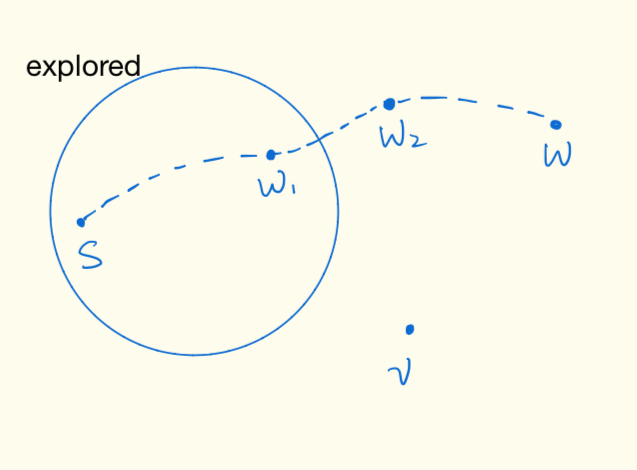
\includegraphics[scale = 0.35]{p1.png}
  \end{center}
  \tab\\
  Denote the subpath from $s$ to $w_1$ in $\Delta(s, w)$ as $p(s, w_1)$, subpath from $s$ to $w_2$ in $\Delta(s, w)$ as $p(s, w_2)$, and subpath $w_2$ to $w$ as $p(w_2, w)$. Based on \texttt{Definition 2.2 Prefix of Path}, $p(s, w_1)$ is a prefix of $\Delta(s, w)$. Since $p(s, w_1)$ is the prefix of the shortest $s-w$ path, then based on \texttt{Lemma 3.1}, $p(s, w_1)$ is the shortest path from $s$ to $w_1$, $\Delta(s, w_1) = p(s, w_1)$, $length(p(s, w_1)) = \delta(w_1)$. 
  \\
  Similarly, since $p(s, w_2) = p(s, w_1) + (w_1, w_2)$, then $p(s, w_2)$ is a prefix of $\Delta(s, w)$, and hence \texttt{Lemma 3.1} implies that $p(s, w_2)$ is the shortest path from $s$ to $w_2$. Then we have: 
  \begin{align*} 
      \Delta(s, w_2) &= p(s, w_2) = p(s, w_1) + (w_1, w_2) \\
      \delta(w_2) &= length(\Delta(s, w_2)) \\
                  &= length(p(s, w_2)) \\
                  &= length(p(s, w_1)) + weight(w_1, w_2)\\
                  &= \delta(w_1) + weight(w_1, w_2) ([E3.5.2])
  \end{align*}
  For $\Delta(s, w)$ we have: 
  \begin{align*}
    \delta(w) &= length(p_w) \\
              &= length(p(s, w_1)) + weight(w_1, w_2) + length(p(w_2, w)) \\
              &= \delta(w_1) + weight(w_1, w_2) + length(p(w_2, w))
  \end{align*}
  Since all edge weights are non-negative, then: 
  \\\\
    \tab $\delta(w_2) = \delta(w_1) + weight(w_1, w_2) \leq \delta(w)$ ([E3.5.3])
  \\\\
  Since $w_1 \in explored_{k+2}$, there are two cases to consider: $w_1 =u_{k+1}$ and $w_1 \neq u_{k+1}$. We will prove P(k+1) under both cases below. 
  \\\\
  \texttt{Case 1: $w_1 = u_{k+1}$}
  \\
  Since $\delta(w_2) = \delta(w_1) + weight(w_1, w_2) \leq \delta(w)$ and all edge weights are non-negative, then $\delta(w_1) \leq \delta(w)$. When $w_1 = u_{k+1}$, we have $\delta(u_{k+1}) \leq \delta(w)$. Since $dist_{k+2}[u_{k+1}] > \delta(w)$ and $\delta(u_{k+1}) \leq \delta(w)$, we have $\delta(u_{k+1}) < dist_{k+2}[u_{k+1}]$.
  \\
  Suppose the node right before $u_{k+1}$ in $\Delta(s, u_{k+1})$ is $w_3$. We know $length(\Delta(s, u_{k+1})) = length(p(s, w_3)) + weight(w_3, u_{k+1}))$, where $p(s, w_3)$ is the prefix of $\Delta(s, u_{k+1})$. Based on \texttt{Lemma 3.1}, we know $length(p(s, w_3)) = \delta(w_3)$. Hence: 
  \begin{align*}
    \delta(u_{k+1}) &= length(p(s, w_3)) + weight(w_3, u_{k+1})) \\
                    &= \delta(w_3) + weight(w_3, u_{k+1}) \\
                    &< dist_{k+2}[u_{k+1}]
  \end{align*}
  i.e.
  \begin{align*}
    dist_{k+2}[u_{k+1}] > \delta(w_3) + weight(w_3, u_{k+1}) ([E3.5.6])
  \end{align*}
  Based on the construction, $w_2$ is the first node along $\Delta(s,w)$, $w_1$ is right before $w_2$ in the path, $w_3$ is right before $w_1 = u_{k+1}$ in the path, then $w_3 \in explored_{k+2}$. Assume $w_3$ is explored during the $j^{th}$ iteration. Then based on \texttt{Lemma 3.4}, we have: 
  \begin{align*}
    dist_{k+2}[u_{k+1}] \leq dist_j[w_3] + weight(w_3, u_{k+1}) ([E3.5.7])
  \end{align*}
  The induction hypothesis implies $dist_{j+1}[w_3] = \delta(w_3)$. For $dist_{j+1}[w_3]$ we have: 
  \begin{align*}
    dist_{j+1}[w_3] &= min(dist_j[w_3], dist_j[w_3] + weight(w_3, w_3)) \\
                   &= min(dist_j[w_3], dist_j[w_3] + 0) \\
                   &= dist_j[w_3]
  \end{align*}
  Hence $dist_j[w_3] = \delta(w_3)$, combine with [E3.5.7], we have: 
  \begin{align*}
    dist_{k+2}[u_{k+1}] \leq \delta(w_3) + weight(w_3, u_{k+1}) ([E3.5.8])
  \end{align*}
  The equation [E3.5.8] contradicts with equation[E3.5.6]. Hence by the principle of prove by contradiction, (L2) holds when $w_1 = u_{k+1}$. 
  \\\\

  \texttt{Case 2}: $w_1 \neq u_{k+1}$
  \\ 
  Since $w_1 \in explored_{k+2}$ and $w_1 \neq u_{k+1}$, $w_1$ is explored before the $(k+1)^{th}$ iteration. i.e., $w_1 \in explored_{k+1}$. Suppose $w_1$ is being explored during the $i^{th}$ iteration, $i < k+1$, then based on the algorithm, the value of $dist_{i+1}[w_1]$ is calculated as: 
  \begin{align*}
        dist_{i+1}[w_1] &= min(dist_{i}[w_1], dist_{i}[w_1] + weight(w_1,w_1)) \\
                        &= min(dist_{i}[w_1], dist_{i}[w_1] + 0)\\
                        &= min(dist_{i}[w_1], dist_{i}[w_1])\\
                        &= dist_{i}[w_1]
  \end{align*}
  Since the induction hypothesis implies that $dist_{i+1}[w_1] = \delta(w_1)$, then $dist_i[w_1] = \delta(w_1)$. 
  \\
  Since $w_1$ has an edge to $w_2$, then $dist_{i+1}[w_2]$ must have been updated according as follows: 
  \begin{align*}
     dist_{i+1}[w_2] &= min(dist_i[w_2], dist_i[w_1] + weight(w_1,w_2)) \\
                     &= min(dist_i[w_2], \delta(w_1) + weight(w_1, w_2))
  \end{align*}
  Based on [E3.5.2] we know that $\delta(w_2) =  \delta(w_1) + weight(w_1, w_2)$, then $dist_{i+1}[w_2] = min(dist_i[w_2], \delta(w_2))$. If $dist_i[w_2] = \infty$, then $dist_{i+1}[w_2] = min(dist_i[w_2], \delta(w_2)) = \delta(w_2)$. If $dist_i[w_2] \neq \infty$, then based on \texttt{Lemma 3.2}, $dist_i[w_2]$ is the length of some $s-w_2$ path. Since $\delta(w_2) \leq length(p), \forall p \in path(s, w_2)$, then $dist_{i+1}[w_2] = min(dist_i[w_2], \delta(w_2)) = \delta(w_2)$. Hence in either cases, we conclude that $dist_{i+1}[w_2] = \delta(w_2)$. 
  \\
  Since $dist_{i+1}[w_2] = \delta(w_2)$ and $i < k+1$, then based on \texttt{Lemma 3.3}, we have:
  \begin{align*}
  dist_{k+1}[w_2] = dist_{i+1} = \delta(w_2) ([E3.5.4])
  \end{align*}
  Based on our assumption, at the beginning of the $(k+1)^{th}$ generation, $u_{k+1}, w_2 \notin explored_{k+1}$ and $u_{k+1}$ is selected by the algorithm, then we must have $dist_{k+1}[w_2] \geq dist_{k+1}[u_{k+1}]$. For $dist_{k+2}[u_{k+1}]$ we have: 
  \begin{align*}
  dist_{k+2}[u_{k+1}] &= min(dist_{k+1}[u_{k+1}], dist_{k+1}[u_{k+1}] + weight(u_{k+1}, u_{k+1})) \\
                      &= min(dist_{k+1}[u_{k+1}], dist_{k+1}[u_{k+1}] + 0) \\
                      &= dist_{k+1}[u_{k+1}] 
  \end{align*}
  Hence $dist_{k+1}[w_2] \geq dist_{k+2}[u_{k+1}]$. Combine with [E3.5.4], [E3.5.3] we have: 
  \begin{align*}
    dist_{k+1}[w_2] &\geq dist_{k+2}[u_{k+1}] (\\
    dist_{k+1}[w_2] &= dist_{i+1} = \delta(w_2) (from [E3.5.4]) \\
    \delta(w) &\geq \delta(w_2) = \delta(w_1) + weight(w_1, w_2)(from [E3.5.3])
  \end{align*}
  Hence $\delta(w) \geq dist_{k+2}[u_{k+1}]$, which contradicts with [E3.5.1]. Hence by the principle of prove by contradiction, when $w_1 \neq u_{k+1}$, $dist_{k+2}[u_{k+1}] \leq \delta(w), \forall w \in unexplored_{k+2}$. 
  \\
  (L2) holds for $u_{k+1}$. 
  \\
  \item (L3) $dist_{k+2}[u_{k+1}] = \delta(u_{k+1})$
  \\\\
  We will prove this by contradiction. 
  \\
  Since (L1) proves $dist_{k+2}[u_{k+1}] \neq \infty$, then \texttt{Lemma 3.2} implies that $dist_{k+2}[u_{k+1}]$ is the length of some $s-u_{k+1}$ path, denote as $p$. Suppose there is a $s-u_{k+1}$ path $p'$ that's shorter than $p$, i.e, $dist_{k+2}[u_{k+1}] > length(p')$([E3.5.9]). Suppose the node right before $u_{k+1}$ in $p'$ is $v'$. Then we know: 
  \begin{align*}
  length(p') &= length(p(s, v')) + weight(v', u_{k+1}) \\
  length(p') &< dist_{k+2}[u_{k+1}]
  \end{align*}
  , where $p(s, v')$ is the prefix of $p'$ from $s$ to $v'$. Hence: 
  \begin{align*}
   dist_{k+2}[u_{k+1}] > length(p(s, v')) + weight(v', u_{k+1}) 
  \end{align*}
  Based on the definition of shortest path, $length(p(s, v')) \geq \delta(v')$, then we have: 
  \begin{align*}
   dist_{k+2}[u_{k+1}] > \delta(v') + weight(v', u_{k+1}) ([E3.5.10])
  \end{align*}
  There are two cases to consider: (1) $v' \in explored_{k+2}$; (2) $v' \notin explored_{k+2}$
  \\\\
  \texttt{Case(1): $v' \in explored_{k+2}$}
  \\
  Suppose $v'$ is explored during the $i^{th}$ iteration. Then \texttt{Lemma 3.4} implies: 
  \begin{align*}
    dist_{k+2}[u_{k+1}] \leq dist_i[v'] + weight(v', u_{k+1}) ([E3.5.11])
  \end{align*}
  The induction hypothesis implies $dist_{i+1}[v'] = \delta(v')$, and for $dist_{i+1}[v']$ we have: 
  \begin{align*}
    dist_{i+1}[v'] &= min(dist_i[v'], dist_i[v'] + weight(v', v')) \\
                   &= min(dist_i[v'], dist_i[v'] + 0) \\
                   &= dist_i[v']
  \end{align*}
  Hence $dist_i[v'] = \delta(v')$. Combining [E3.5.11], we have: 
  \begin{align*}
    dist_{k+2}[u_{k+1}] \leq \delta(v') + weight(v', u_{k+1}) ([E3.5.12])
  \end{align*}
  Hence equation [E3.5.12] contradicts with equaltion [E3.5.10]. By the principle of prove by contradiction, (L3) holds when $v' \in explored_{k+2}$. 
  \\\\
  \texttt{Case(2): $v' \notin explored_{k+2}$}
  \\
  Since $length(p') = length(p(s, v')) + weight(v', u_{k+1})$, $p(s, v)$ is the prefix of $p'$ from $s$ to $v'$, then based on the definition of shortest path, $length(p(s, v')) \leq \delta(v')$, and thus $\delta(v') + weight(v', u_{k+1}) \leq length(p(s, v')) + weight(v', u_{k+1}) = length(p')$. Since all edge weights are non-negative, then $\delta(v') \leq length(p')$.
  \\
  Since $v' \notin explored_{k+2}$, i.e., $v' \in unexplored_{k+2}$, based on proof of (L2), $dist_{k+2}[u_{k+1}] \leq \delta(v')$. Since $dist_{k+2}[u_{k+1}] \leq \delta(v')$ and $\delta(v') \leq length(p')$, then $dist_{k+2}[u_{k+1}] \leq length(p')$, which contradicts with our assumption ([E3.5.9]). Hence by the principle of prove by contradiction, (L3) holds when $v' \notin explored_{k+2}$. 
  \\
  Since we have proved (L3) for both cases, then (L3) holds for P(K+1). 
  \end{enumerate}
\end{itemize}
Since we have proved (L1)(L2)(L3) forall nodes in $explored_{k+1}$ after the $(k+1)^{th}$ iteration, P(k+1) holds. Then by the principle of prove by induction, \texttt{Lemma 3.5} holds. 
\end{proof}

\begin{proof}\textbf{Prove of Correctness}
\\\\
By applying \texttt{Lemma 3.5(L3)} to the last iteration of the algorithm, we obtained that for all nodes $n$ in the explored list, $dist[n]$ is indeed the shortest path distance value from source $s$ to $n$, hence Dijkstra's algorithm indeed calculates the shortest path distance value from the source $s$ to each node $n \in g$. 
\end{proof}
\end{document}


